\documentclass[submit]{harvardml}

% Put in your full name and email address.
\name{Weiyi Chen}
\email{wec427@g.harvard.edu}

% List any people you worked with.
\collaborators{%
    None
}

% You don't need to change these.
\course{CS181-S16}
\assignment{Assignment \#5}
\duedate{April 24, 2016}

\usepackage[OT1]{fontenc}
\usepackage[colorlinks,citecolor=blue,urlcolor=blue]{hyperref}
\usepackage[pdftex]{graphicx}
\usepackage{subfig}
\usepackage{fullpage}
\usepackage{palatino}
\usepackage{mathpazo}
\usepackage{amsmath}
\usepackage{amssymb}
\usepackage{color}
\usepackage{todonotes}
\usepackage{listings}
\usepackage{common}
\usepackage{bm}
\usepackage{enumitem}

\usepackage[mmddyyyy,hhmmss]{datetime}

\definecolor{verbgray}{gray}{0.9}

\lstnewenvironment{csv}{%
  \lstset{backgroundcolor=\color{verbgray},
  frame=single,
  framerule=0pt,
  basicstyle=\ttfamily,
  columns=fullflexible}}{}

\begin{document}
\begin{center}
{\Large Homework 5: EM for a Simple Topic Model}\\
\end{center}

There is a mathematical component and a programming component to this homework.
Please submit ONLY your PDF to Canvas, and push all of your work to your Github
repository. If a question requires you to make any plots, please
include those in the writeup.

\begin{mdframed}[style=exampledefault]
\textbf{Background:} In this homework, you will implement a very simple kind of topic model.  Latent Dirichlet allocation, as we discussed in class, is a topic model in which each document is composed of multiple topics.  Here we will make a simplified version in which each document has just a single topic.  As in LDA, the vocabulary will have~$V$ words and a topic will be a distribution over this vocabulary.  Let's use~$K$ topics and the~$k$th topic is a vector~$\bbeta_k$, where~${\beta_{k,v}\geq 0}$ and~${\sum_v \beta_{k,v}=1}$.  Each document can be described by a set of word counts~$\boldw_{d}$, where~$w_{d,v}$ is a nonnegative integer.  Document~$d$ has~$N_d$ words in total, i.e.,~${\sum_v w_{d,v}=N_d}$.  Let's have the unknown overall mixing proportion of topics be~$\btheta$, where~${\theta_k\geq 0}$ and~${\sum_k\theta_k=1}$.  Our generative model is that each of the~$D$ documents has a single topic~${z_d\in \{1,\ldots,K\}}$, drawn from~$\btheta$; then, each of the words is drawn from~$\bbeta_{z_d}$.

\end{mdframed}

%%%%%%%%%%%%%%%%%%%%%%%%%%%%%%%%%%%%%%%%%%%%%
% Problem 1
%%%%%%%%%%%%%%%%%%%%%%%%%%%%%%%%%%%%%%%%%%%%%
\begin{problem}[Complete Data Log Likelihood, 4 pts]

Write the complete-data log likelihood~$\ln p(\{z_d,\boldw_d\}^D_{d=1}\given\btheta, \{\bbeta_k\}^K_{k=1})$. It may be convenient to write~$z_d$ as a one-hot coded vector~$\boldz_d$.


\end{problem}
\subsection*{Solution}

Write $z_d$ as a one-hot coded vector $\boldz_d$, in which a particular element of $\boldz_d$ is equal to 1 and all other elements are equal to 0. The values of $\boldz_d$ therefore satisfy $z_{d,k} \in \{0,1\}$ and $\sum_k z_{d,k} = 1$. Since $\boldz_d$ uses a 1-of-K representation, we can also write its distribution in the form
$$ p(\boldz_d) = \prod_{k=1}^K \theta_k^{z_{d,k}} $$ 
The conditional distribution of $\boldw_d$ given a particular value for $\boldz_d$ is
$$ p(\boldw_d \given \boldz_d) = \prod_{k=1}^K \left( \frac{\sum_{v=1}^V{w_{d,v}\beta_{k,v}}}{N_d} \right)^{z_{d,k}} $$
The joint distribution is given by $p(\boldz_d)p(\boldw_d\given\boldz_d)$, and the marginal distribution of $\boldw_d$ is then obtained by summing the joint distribution over all possible states of $\boldz_d$ to give
$$ p(\boldw_d) = \sum_{\boldz_d} p(\boldz_d)p(\boldw_d\given\boldz_d) = \sum_{k=1}^K z_{d,k} \theta_k \left( \frac{\sum_{v=1}^V{w_{d,v}\beta_{k,v}}}{N_d} \right) $$
The log likelihood is 
$$ \ln p(\boldw_d) = \ln \sum_{k=1}^K \left(z_{d,k} \theta_k \sum_{v=1}^V{w_{d,v}\beta_{k,v}}\right) - \ln N_d $$
The complete-data log likelihood is 
$$ \ln p(\boldw) = \sum_{d=1}^D \left[ \ln \sum_{k=1}^K \left(z_{d,k} \theta_k \sum_{v=1}^V{w_{d,v}\beta_{k,v}}\right) - \ln N_d \right]$$
Actually $N_d$ is irrelevant at latter steps, it can be reduced to 
$$ \ln p(\boldw) = \sum_{d=1}^D \left[ \ln \sum_{k=1}^K \left(z_{d,k} \theta_k \sum_{v=1}^V{w_{d,v}\beta_{k,v}}\right) \right]$$

\newpage
\begin{problem}[Expectation Step, 5pts]

Introduce estimates~$q(\boldz_d)$ for the posterior over the hidden variables~$\boldz_d$.  What did you choose and why?  Write down how you would determine the parameters of these estimates, given the observed data~$\{\boldw_d\}^D_{d=1}$ and the parameters~$\btheta$ and~$\{\bbeta_k\}^K_{k=1}$.

\end{problem}
\subsection*{Solution}

The posterior probability of estimates $q(z_d)$ can be found using Bayes' theorem (note unbold $z_d$ still refers to the original problem setting $z_d \in \{1,\dots,K\}$,

$$ q(z_d = k) \equiv p(z_d=k \given \boldw_d) = \frac{p(z_d=k)p(\boldw_d\given z_d=k)}{\sum_{j=1}^Kp(z_d=j)p(\boldw_d\given z_d=j)} = \frac{\theta_k z_{d,k} \sum_{v=1}^V{w_{d,v}\beta_{k,v}} }{\sum_{j=1}^K{\left( \theta_j z_{d,j} \sum_{v=1}^V{w_{d,v}\beta_{j,v}} \right)}} $$

The reason is quite obvious stated above, the posterior estimates are defined as $p(z_d=k \given \boldw_d)$. And we shall view $\theta_k$ as the prior probability of $z_d=k$, and using the Bayes' theorem as well as the formula of $p(\boldw_d\given z_d=k)$ from Problem 1. As we shall see, $q(z_d)$ can be viewed as the responsibility that component $k$ takes for 'explaining' the observation $\boldw_d$. Note the above formula applies to all $d = 1,\dots, D$.

\newpage

\begin{problem}[Maximization Step, 5pts]
With the~$q(\boldz_d)$ estimates in hand from the E-step, derive an update for maximizing the expected complete data log likelihood in terms of~$\btheta$ and~$\{\bbeta_k\}^K_{k=1}$.

\begin{enumerate}[label=(\alph*)]
    \item Derive an expression for the expected complete data log likelihood for fixed $\gamma$'s. 
    \item Find a value of $\theta$ that maximizes the expected complete data log likelihood derived in (a). You may find it helpful to use Lagrange multipliers in order to force the constraint $\sum \theta_k = 1$. Why does this optimized $\theta$ make intuitive sense?
    \item Apply a similar argument to find the value of $\beta_{k, v}$ that maximizes the expected complete data log likelihood. 
\end{enumerate}

\end{problem}
\subsection*{Solution}

\subsubsection*{(a)}

As stated on piazza, $\gamma_{d,k} \equiv q(z_{d,k})$. Observing the conclusions of Problem 1 and 2, we find denominators of $q(z_{d,k})$ in Problem 2 and the left part inside the summation of $d$ in Problem 1 are the same, therefore we can replace using formula
$$ \sum_{j=1}^K{\left( \theta_j z_{d,j} \sum_{v=1}^V{w_{d,v}\beta_{j,v}} \right)} = \frac{\theta_k z_{d,k} \sum_{v=1}^V{w_{d,v}\beta_{k,v}}}{\gamma_{d,k}} $$
and derive the expected complete-data log likelihood as 
$$ \ln p(\boldw) = \sum_{d=1}^D \left[ \ln \frac{\theta_k z_{d,k} \sum_{v=1}^V{w_{d,v}\beta_{k,v}}}{\gamma_{d,k}} \right]$$

\subsubsection*{(b)}

We maximize the conclusion from part (a) with respect to the mixing coefficients $\theta_k$. Here we must take account of the constraint $\sum_{k=1}^K \theta_k = 1$. This can be achieved using a Lagrange multiplier and maximizing the following quantity
$$ \ln p (\boldw) + \lambda \left( \sum_{k=1}^K \theta_k - 1 \right) $$
which gives
$$ 0 = \sum_{d=1}^D \frac{\gamma_{d,k}}{\theta_k} + \lambda $$
If we now multiply both sides by $\theta_k$ and sum over $k$ making use of the constraint, we find $\lambda = -D$. Using this to eliminate $\lambda$ and rearranging we obtain
$$ \theta_k = \frac{\sum_{d=1}^D \gamma_{d,k}}{D} $$ 
This optimized $\theta$ makes intuitive sense because the mixing coefficient for the $k$-th component is given by the average responsibility which that component takes for explaining the data points.

Further speaking in this case, this is very intuitive because the numerator is just counting/summing all the contributions to the $k$-th topic from different documents, and then normalizing it by their sum as of $D$.

\subsubsection*{(c)}

Similarly we maximize the conclusion from part (a) with respect to $\beta_{k,v}$. Here we will take account of the constrant $\sum_{v=1}^V \beta_{k, v} = 1$. Again this can be achieved using a Lagrange multiplier and maximizing the following quantity 
$$ \ln p (\boldw) + \lambda \left( \sum_{v=1}^V \beta_{k,v} - 1 \right) $$
which gives
$$ 0 = \sum_{d=1}^D \gamma_{d,k} \frac{w_{d,v}}{\sum_{v'=1}^Vw_{d,v'}\beta_{k,v'}} + \lambda $$
If we now multiply both sides by $\beta_{k,v}$ and denote 
$$ \alpha_{d,k,v} = \frac{w_{d,v}\beta_{k,v}}{\sum_{v'=1}^Vw_{d,v'}\beta_{k,v'}} $$
as another probability indicating the responsibility of each word in document $d$ contributes to $k$ among all the words in the vocabulary. With this introduction, we sum over $v$ making use of the constraint, we find $\lambda = -D$. Using this to elimate $\lambda$ and rearranging we obtain 
$$\beta_{k,v} = \frac{\sum_{d=1}^D \alpha_{d,k,v} \gamma_{d,k}}{\sum_{d=1}^D \gamma_{d,k}}$$
which applies to all $k$ and $v$.

\newpage

\begin{problem}[Implementation, 10pts]
Implement this expectation maximization algorithm and try it out on some text data.  In order for the EM algorithm to work, you may have to do a little preprocessing.  

$\linebreak$
\noindent The starter code loads the text data as a numpy array that is $5224951 \times 3$ in size. As shown below, the first number in the numpy array represents the document\_id, the second number represents a word\_id, and the third number is the count the word appears. 


$$ [\text{doc\_id, word\_id, count}]$$

\noindent A dictionary of the mappings between word\_ids and words is also provided. The full dataset description can be found at \url{http://kdd.ics.uci.edu/databases/nsfabs/nsfawards.data.html}.\\ 

\noindent Plot the objective function as a function of iteration and verify that it never increases. Try different numbers of topics and report what topics you find by, e.g., listing the most likely words. 

\end{problem}
\subsection*{Solution}

\subsubsection*{(1) \# topics = 10}

The objective function as a function of iteration is plotted as Figure 1, it never increases. Actually 500 iterations is too many since latter iterations did not help improve reduce the objective a lot. So when continue trying with different number of topics, I will use 100 as the the number of iterations and re-plot to verify. 

\begin{figure}[h]
    \centering
    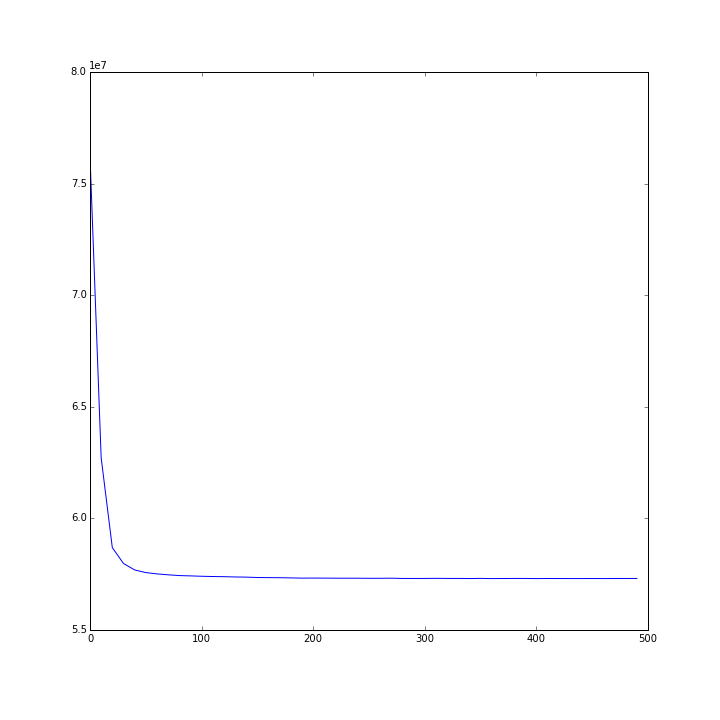
\includegraphics[scale=0.45]{prob4.png}
    \caption{Objective vs. iteration, \# topics = 10}
\end{figure}

The topics are presented via the most likely words below, which is the output of my program

\begin{lstlisting}
Topic 0: research study data project species social important
Topic 1: students science project research laboratory program undergraduate
Topic 2: protein cell cells molecular proteins dna gene
Topic 3: materials high optical research magnetic properties laser
Topic 4: chemistry research chemical molecular reactions organic studies
Topic 5: data study project ocean water climate ice
Topic 6: research university support award program dr science
Topic 7: theory problems study research equations mathematical methods
Topic 8: research systems design system data control computer
Topic 9: research flow phase project process materials model
\end{lstlisting}

The result is obviously correct, e.g. top words of topic 2 are mostly related to Biology, and top words of topic 4 are mostly related to Chemistry.

\subsubsection*{(2) \# topics = 20}

Let's try a larger number of topics, to see whether it can make the topic words more specific to some field. The obj vs. iteration plot as Figure 2 still keeps decreases and is almost flat at the end.

\begin{figure}[h]
    \centering
    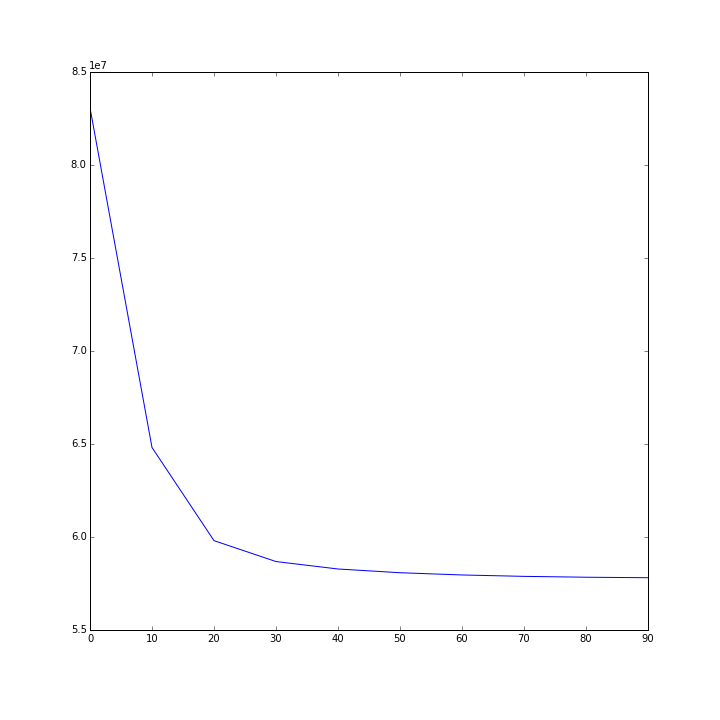
\includegraphics[scale=0.45]{prob4-20.png}
    \caption{Objective vs. iteration, \# topics = 20}
\end{figure}

The topics with top words - 

\begin{lstlisting}
Topic 0: species plant populations study population research genetic
Topic 1: research project social study data economic policy
Topic 2: research climate global change months support year
Topic 3: design systems system research control performance network
Topic 4: cells cell system development brain mechanisms function
Topic 5: chemistry research molecular reactions chemical properties electron
Topic 6: science project students teachers mathematics education school
Topic 7: data study ice project ocean seismic earthquake
Topic 8: research university dr project award support program
Topic 9: data research provide important project study dr
Topic 10: laboratory students equipment research computer analysis chemistry
Topic 11: materials research high phase optical devices properties
Topic 12: research students program engineering science graduate undergraduate
Topic 13: water carbon chemical processes organic production environmental
Topic 14: protein proteins dna gene molecular genes cell
Topic 15: methods problems research data models algorithms analysis
Topic 16: conference workshop research support held international scientists
Topic 17: theory problems study equations research mathematical geometry
Topic 18: model models flow study systems dynamics numerical
Topic 19: high data solar measurements resolution imaging observations
\end{lstlisting}

The topic becomes easier to identify as well, this is quite intuitive since more topics let the documents be separated into more directories, and each directory would be more specific to some field, which makes it easier to be identified.

\subsubsection*{(3) \# topics = 5}

Just take a try at a smaller number, to verify our conclusion from part (2) that less number of topics would result in difficulties to identify its underlying topic.

Firstly verify the objective vs. iteration plot as of Figure 3.

\begin{figure}[h]
    \centering
    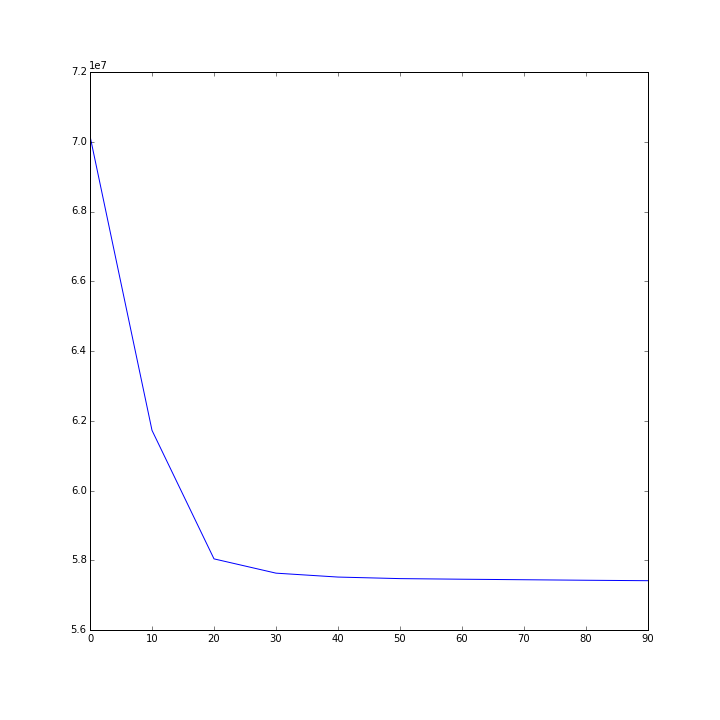
\includegraphics[scale=0.45]{prob4-5.png}
    \caption{Objective vs. iteration, \# topics = 5}
\end{figure}

Then look at the top words as follows

\begin{lstlisting}
Topic 0: research data study project species important provide
Topic 1: research students science university project program support
Topic 2: research high study materials project surface properties
Topic 3: research theory systems problems design project methods
Topic 4: molecular protein cell cells studies research proteins
\end{lstlisting}

It is still possible to identify Topic 4 is Biology and others are quite difficult, as expected.

\newpage
\begin{problem}[Calibration, 1pt]
Approximately how long did this homework take you to complete?
\end{problem}
12 hours.

\end{document}